

\begin{figure}[t]
\centering
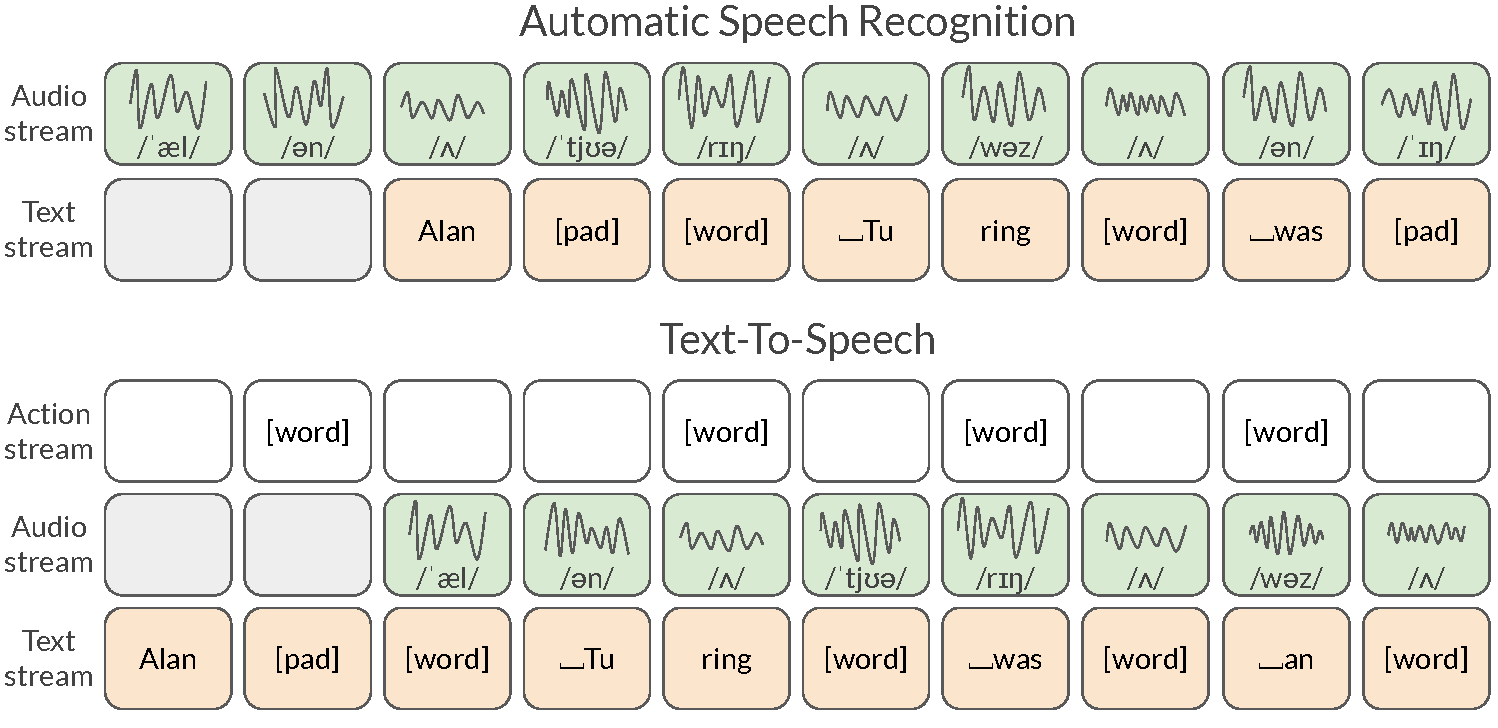
\includegraphics[width=.7\textwidth]{figures/Figure_time_delay-3_cropped.pdf}
\caption{\textbf{Delayed streams modeling for speech-text tasks}. Depending on which stream is delayed with respect to the other, we solve either an ASR or a TTS task. For TTS, we further need an action stream for the model to let us know when it is ready to receive a new word.
}
\label{fig:concept}
\end{figure}

\section{Method}

\label{sec:modeling}
\textbf{Notation.}\ 
We wish to solve a sequence-to-sequence task between two domains 
$\mathcal{X}$ and $\mathcal{Y}$. Each domain consists of sequences of vectors of all possible lengths, e.g. 
\begin{equation}
\label{eq:domain_def}
    \mathcal{X} = \bigcup_{T \in \nats} \{ (X_{t}) \in \reals^{T \times d }\}, \qquad
    \mathcal{Y} = \bigcup_{T' \in \nats} \{ (Y_{t'}) \in \reals^{T' \times d' }\}.
\end{equation}
In the case where either $X_t$ or $Y_t$  is discrete-valued, we can use a one-hot representation for it in Eq.~\eqref{eq:domain_def}.
We assume that we are given a joint probability distribution over the outer product domain $\mathcal{X}\times \mathcal{Y}$, and that we have
the random variables $X \in \mathcal{X}$ and $Y \in \mathcal{Y}$, along with the joint distribution \begin{equation}\proba{X, Y} = p(X ,Y). \end{equation}
We also introduce $T \in \nats$ (resp.\ $T'$) the random variable indicating
the length of $X$ (resp.\ $Y$), along with the marginals $p(X)$ and $p(Y)$. For any sequence $Z$, and index $t$, we denote $Z_{<t} = (Z_1, \ldots, Z_{t-1})$, %
potentially empty if $t \leq 0$. We similarly define $Z_{\leq t}$, $Z_{\geq t}$, and $Z_{> t}$.

\textbf{Sequence-to-sequence as joint modeling.}\ 
Let's assume for this paragraph that $\mathcal{X}$ is the set of all possible monophonic waveforms sampled at 24 kHz,
and $\mathcal{Y}$ is made of sequences of one-hot encoded vectors over a set of words.
Intuitively, we assume there exists a coupling $p(X, Y)$ such that $p(X, Y)$ is high
if $Y$ represents the transcription of $X$, or conversely, if $X$ represents a speech utterance
of the text given by $Y$.
Formally, the task of ASR corresponds to sampling from the distribution $\proba{Y | X}$, 
while the task of TTS corresponds to sampling from the distribution $\proba{X | Y}$.
Thus, each task can be solved by accurately estimating both probability distributions,
\begin{equation}
    \label{eq:estimate}
    q(X, Y)\approx \proba{Y | X}, \qquad q'(Y, X) \approx \proba{X | Y}.
\end{equation}

For simplicity, we now only focus on estimating $\proba{Y|X}$, the inverse task being obtained by
exchanging the definition of $X$ and $Y$. We thus call $\mathcal{X}$ the input domain, and $\mathcal{Y}$ the output domain.

\textbf{Auto-regressive modeling of $Y$.}\ 
A good candidate for estimating $\proba{Y | X}$ is auto-regressive modeling, with a Transformer model~\citep{attentionvaswani}, under the extra assumption that the output domain $\mathcal{Y}$ can be discretized. Thus, one would estimate
\begin{equation}
    q(y | X, Y_{< t}) \approx \proba{Y_t=y | X, Y_{<t}}.
\end{equation}

One can then sample $Y$ auto-regressively, knowing $X$.
Due to the lack of explicit structure between the time grid $t$ of $X$ and $t'$ of $Y$,
one would usually condition on the entirety of $X$, e.g.\ when using Transformer based models, 
either by prefixing the entire sequence
$X$ before the generation $Y$, or by providing $X$ through cross-attention layers, which is mathematically equivalent. 
This forbids the use of the model in a streaming fashion, as the entire input signal $X$ must be known ahead of time, and cannot be extended once the generation of $Y$ has started.
Such methods often require explicit and manual chunking and stitching operations, which also reduces their ability to be efficiently batched. Conversely, aligning $X$ and $Y$ to the same frame rate allows for batched streaming inference.

\textbf{Aligning sequences for streaming prediction.}
We assume that both domains $\mathcal{X}$ and $\mathcal{Y}$ can share the same time grid,
e.g.\ $(X_t)\in\reals^{T \times d}$ and $(Y_t)\in\reals^{T \times d'}$. 
We call two such aligned sequences \emph{streams}. 
Then one can simply model%
\begin{equation}
\label{eq:q_aligned}
    \qal{y | X_{\leq t}, Y_{< t}} \approx \proba{ Y_t = y|X_{\leq t}, Y_{< t}}.
\end{equation}
Given $X\sim p(X)$, we sample auto-regressively from Eq.~\eqref{eq:q_aligned}, \emph{with a streaming context} $X$,
\begin{equation}
\label{eq:sample_ty}
   \tY_1 \sim  \qal{\tY_1 | X_1}, \qquad
   \tY_t \sim \qal{\tY_t | X_{\leq t}, \tY_{< t}}.
\end{equation}
We would want that given $X\sim p(X)$, then $(X, \tY)\sim(X, Y)$,
so that in particular $\proba{\tY | X} \approx \proba{Y | X}$.
However this needs not be the case unless certain conditions are met.

\textbf{The importance of causality.}\ 
In particular, for $(X, \tY)\sim(X, Y)$ to be true,
$Y_{> t}$ must be independent of $X_{> t}$, knowing $X_{\leq t}$.
To realize that, one can look at a simple counter-example taking
$X_t \sim \mathcal{B}(0.5)$ independent Bernoulli variables,
and $Y_t = X_t \oplus X_{t+1}$ the XOR of $X_t$ and $X_{t+1}$.
Clearly $\proba{Y_t | X_{\leq t}, Y_{< t}} \sim \mathcal{B}(0.5)$ for all $t$, yet, given $X = (0, 1)$, one would have 
\begin{equation*}
Y_1 = 1 \quad\text{a.s.},\qquad \tY_1 \sim \mathcal{B}(0.5).
\end{equation*}
Thus $Y | X$ and $\tY | X$ have different distributions. Intuitively, given that we do not sample $X$ but teacher-force real-world data, we must ensure that when sampling $\tY_t$, no future value of $X_{>t}$ might end up in ``contradiction'' with the value we sampled.

\textbf{Delaying the output stream.}\ 
In practice, this is achieved by delaying the output stream $Y_t$ by a number of steps $\tau > 0$.
Thus, we replace Eq.~\eqref{eq:q_aligned} by
\begin{equation}
\label{eq:q_delayed}
\qdel{y | X_{\leq t + \tau}, Y_{< t}} \approx \proba{ Y_t=y |X_{\leq t +\tau}, Y_{< t}},
\end{equation}
and define $\tY^\tau$, similarly to the procedure described in Eq.~\ref{eq:sample_ty}.
Perfect independence is hard to achieve: in the case of ASR, a named entity might be ambiguous without context, and only future development in a discussion would resolve this ambiguity. Taking $\tau = T$ recovers the prefixing or cross-attention approaches presented earlier. In practice, there is a trade-off between the level of independence of $Y_t$ with $X_{> t + \tau}$, and the latency of the method.

\begin{figure}
\centering
\begin{minipage}[t]{.42\textwidth}
\centering
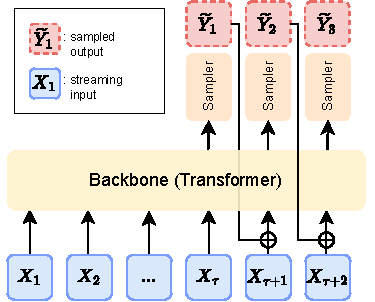
\includegraphics[width=0.9\textwidth]{figures/DSM_arch.drawio-4.pdf}
\caption{\textbf{DSM Architecture}. %
\looseness=-1
Transformer is fed %
with the streaming input $X_t$. After a delay $\tau$, a sampler is fed with the output of the backbone samples $\tY_t$. At the next step, the backbone receives both the sampled value and next streaming input, whose embeddings are summed.}
\label{fig:architecture}
\end{minipage}\hspace{.03\textwidth}%
\begin{minipage}[t]{0.55\textwidth}
\centering
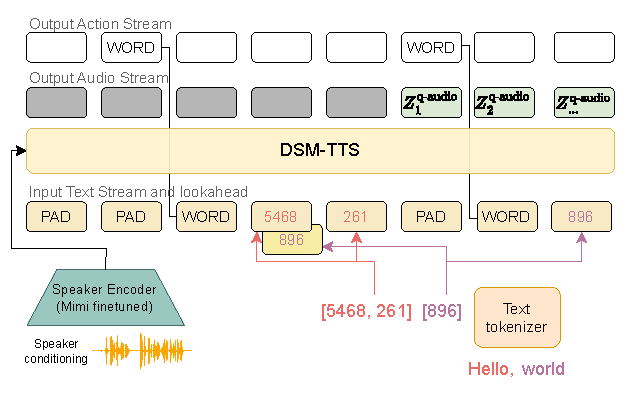
\includegraphics[width=0.9\textwidth]{figures/TTS_figure.drawio-4-1-2.pdf}
\caption{\textbf{DSM-TTS inference}.
The input words ``{\color{BrickRed}Hello,} {\color{Orchid}world}'' are tokenized. Until the model action stream outputs a \spectoken{WORD}, it is fed with \spectoken{PAD}. Then the first word's tokens are fed, including a look-ahead text stream. Once a delay $\tau$ (here 5 for illustration purposes) has accumulated, the model also outputs the audio.}
\label{fig:tts_inference}
\end{minipage}
\end{figure}


\looseness=-1
\textbf{Architecture.}\ DSM, depicted in Figure~\ref{fig:architecture}, contains three components:
(i) an auto-regressive backbone, (ii) an input embedder for $X$ and $Y$ into the backbone, and (iii) a sampler for $\tY^\tau$ conditioned on the output of the backbone. 
The backbone can be a Transformer architecture, optionally equipped with cross-attention layers
to provide further non-streaming contextual information.
The embedder for $X$ and $Y$ can be learnt embedding tables in the case where both domains are discrete. The embeddings are summed before going into the backbone. On the output side, we mask the loss on the tokens of $X$ and only compute cross-entropy on $Y$. Finally, the conditional sampler can be a linear layer applied to the output of the backbone to derive logits if $Y$ is discrete. It could also be a flow or diffusion model conditioned on the output of the backbone for the continuous case.

\subsection{Representations of the speech and text domains}
\label{sec:representations}
We demonstrate the DSM framework on ASR and TTS, where the two domains are text and audio. %

\looseness=-1
\textbf{Audio.}\ 
Given a waveform $w \in \reals^{d_s \cdot f_s}$ with the duration in seconds $d_s$ and the sample rate $f_s=24\,\text{kHz}$, we turn it into a more compact latent space using the Mimi codec~\citep{moshi}, giving us
a sequence of tensors $Z^\text{audio} \in \reals^{d_s \cdot f_r \times d_{\text{audio}}}$, 
with a frame rate of $f_r=12.5\,\text{Hz}$.
This latent space is discretized with Residual Vector Quantization~\citep{soundstream} (RVQ), giving us
a set of $Q \in \llbracket 1, 32\rrbracket$ coarse-to-fine discrete values per time step with cardinality $N_a{=}2048$, each coming from one codebook in the RVQ, giving a quantized representation $Z^\text{q-audio} \in \{1, \ldots, N_a\}^{d_s \cdot f_r \times Q}$.


\looseness=-1
\textbf{Text.}\ 
We tokenize text using a vocabulary of $N_t$, specifically trained on speech data transcriptions.
Two tokens have a special meaning: \spectoken{PAD} (indicating the absence of words at this time) and \spectoken{WORD} (indicating the start of a new word following~\citet{moshi}.
Given a transcript, with word-level timestamps, of a waveform of duration $d_s$, its aligned text representation is $Z^\text{text}\in\{1, \ldots N_t\}^{d_s \cdot f_r}$.
For each word in the transcript represented by tokens $(x_1, \ldots, x_n) \in \{1, \ldots, N_t\}^n$ and starting at $s \in \reals^+$ seconds, we
define its start index $i = \mathrm{floor}(s \cdot f_r)$, and store it as $Z^\text{text}_{i} \leftarrow \spectoken{WORD}$, 
$Z^\text{text}_{i+1}\leftarrow x_1$, $Z^\text{text}_{i+2}\leftarrow x_2$, etc. Any step in $Z^\text{text}$ not assigned by a word token is given the special value \spectoken{PAD}. 

\subsection{DSM for automatic speech recognition: DSM-ASR}
\label{sec:dsm_asr}

\looseness=-1
For ASR, we consider $X = Z^\text{q-audio}$  and $Y = Z^\text{text}$. By predicting the word tokens of $Y$, we learn to transcribe audio, while computing the loss on \spectoken{PAD} and \spectoken{WORD} tokens trains the model to predict the precise boundaries of each word. At inference time, we teacher-force the audio tokens of $X$ and sample the full sequence $Z^\text{text}$ to obtain a transcription along with timestamps with a precision of 80ms (frame size). %
This is allowed by the fact that we apply a constant delay to all words in the sequence, meaning we only need to shift the output timestamps back by the same value to recover the true timestamps. %

\looseness=-1
\textbf{Deriving aligned speech-text data.}\ 
We are looking for fine-grained alignment between speech and text, however speech datasets are typically aligned at the level of the sentence~\citep{librispeech}. Conveniently, \texttt{whisper-timestamped}~\citep{lintoai2023whispertimestamped} provides automatic transcriptions with word-level timestamps. We rely on these pseudo-labels for the pretraining phase of \oursASR{}. We then finetune on a mixture of public datasets with ground-truth transcripts (see details in Section ~\ref{sec:training_protocol}), which pose two challenges.
First, the automatic transcriptions extracted by Whisper in pretraining are formatted with capitalization and punctuation, but the level of formatting varies a lot between datasets.
To address this, we train a 300M prefix-LM for automatic formatting, on a dataset of formatted Whisper transcripts. %
A second challenge is that these ground-truth transcripts do not have word-level alignment. We derive those by producing pseudo-transcripts with Whisper, and reconciling them with the formatted transcript using a Dynamic Time Warping algorithm~\citep{giorgino2009computing}.

\textbf{Delay conditioning for inference-time control.}
\looseness=-1
As shown in Section~\ref{sec:dsm_asr_results},  transcription quality is heavily dependent on the delay between audio and text. Thus, training \oursASR{} with a fixed delay requires choosing a latency/quality trade-off beforehand, and retraining a new model for each delay, despite the training task remaining fundamentally the same. To instead control this trade-off at inference, we train \oursASR{} over random delays, sampled for each sequence. %
The model is additionally conditioned on a cosine embedding~\citep{attentionvaswani} of the delay (expressed in milliseconds), added to the inputs. Experiments in Section~\ref{sec:dsm_asr_results} compare this model to the models trained with a fixed delay %
and show that the effective delay precisely respects the conditioning value.

\subsection{DSM for text-to-speech}
\label{sec:dsm_tts}
\looseness=-1
We further apply DSM to TTS, taking $X = Z^\text{text}$, $Y = Z^\text{q-audio}$. We use a stream delay of 1.28s (or 16 steps) on the output audio.
For sampling along the $Q$ dimension in $Z^\text{q-audio}$, we use a RQ-Transformer as a sampler~\citep{rq-transformer, moshi}, i.e.\ a smaller Transformer conditioned on the output of the backbone at each timestep and performing autoregressive modeling along the $Q$ dimension.
All the backbone inputs (generated audio tokens and next word token input) are fed through learnt embeddings and summed.
We are confronted with the problem that the input domain is no longer plain text, but text properly padded for time alignment.
While at train time we can teacher-force the ground-truth padded text, this is not the case for a novel text to synthesize at inference time.

\textbf{Action output stream.}
\looseness=-1
We add an extra stream to the TTS outputs,
whose goal is to predict whether the next input text token will be a \spectoken{WORD} token or not. This special input token indicates that a new word is starting, and that its tokens are going to follow as inputs.
This extra stream controls an inference-time \emph{action}: when predicted by the model, we will feed as input the text tokens for the next word over the next time steps.
While these are being fed, the model is not allowed to output another \spectoken{WORD} action. The action output stream is not fed back into the model as it is redundant with the text stream input.

\looseness=-1
\textbf{Lookahead second text stream.}
The action stream allows the model to predict the next word position,
although the model has no knowledge of its content for making that decision. The delay between text and audio only provides context for the audio generation, however, the decision on where to insert pauses and words has no such context. Given a sequence of words $m_1, m_2, \ldots$, the lookahead text stream feeds the tokens of the words $m_{i + l}$ to the backbone while the primary text feed contains the tokens of words $m_{i}$.

\looseness=-1
\textbf{Speaker conditioning.} 
We provide speaker embeddings for up to 5 speakers.
Each speaker is represented by a 10s audio extract of the same speaker outside of the training segment. Speakers are identified using the diarization tool Pyannote~\citep{Bredin23} in the training data. If more than 5 speakers are present in the segment, only 5 at random are kept for the speaker embeddings. If less than 5 speakers are present, the remaining speaker slots are filled with learnt padding values. Each speaker audio extract is encoded with a \emph{speaker encoder} and results in a speaker embedding with a fixed dimension. We concatenate the speaker embedding from the different speakers, sum them with an absolute positional embedding, and feed them through cross-attention layers to the backbone. The speaker encoder has the same architecture as the encoder of the Mimi codec, and is initialized with its weights. We keep the weights of the convolutional layers frozen for stability, but let its Transformer layers be fine-tuned in an end-to-end fashion with the language model conditioned on it. 

\textbf{Change of turn tokens.}
We indicate change of turns between the first speaker in the speaker embedding, called the \emph{main speaker}, and any other speaker. When the main speaker starts talking, their first word is prefixed with a special \spectoken{MAIN} token in the text stream. When another speaker starts speaking after the main speaker, a special \spectoken{OTHER} token is inserted.
At inference time, we can thus make controllable dialogs by feeding the model with speaker embeddings for the two speakers, and controlling the change of turn by inserting the \spectoken{MAIN} and \spectoken{OTHER} special tokens.

\textbf{Classifier free guidance.}
We use classifier free guidance (CFG) ~\citep{ho2022classifier,audiogen}, both with respect to the speaker conditioning, and also with respect to the text, that is, we replace at inference time the logits for a given timestep $t$ and codebook index $q$, given $\alpha \geq 1$, with
\begin{equation}
\label{eq:cfg}
    l_{t, q} = l^{\emptyset}_{t, q} + \alpha \left(
    l^{\text{text,speaker}}_{t, q} - 
    l^{\emptyset}_{t, q}
    \right),
\end{equation}
where $l^{\emptyset}_{t, q}$ are the logit estimates obtained by feeding no text, action or lookahead inputs to the model, and no speaker embedding, and 
$l^{\text{text,speaker}}_{t, q}$ are the conditioned logits estimates.
No CFG is applied on the action stream logits. The model is trained with an independent dropout of 20\% on the speaker embedding and on the input text. Unless stated otherwise, we use $\alpha = 2$.

An overview of the whole DSM-TTS inference process is shown in Figure~\ref{fig:tts_inference}.
